\section{Recursive Systematic Convolutional Codes:Review}
\label{sec2}

An $(n,k)$ RSC code is a convolutional code generated by using feedback shift registers which has its input bits as part of the codeword. At each time instant it receives an input of $k$ bits and outputs $n$ bits. The output bits are determined by the generator function, which may be written in polynomial notation as  $\Big[1 ~\frac{f(x)}{g(x)}\Big]$. Given the systematic nature of the RSC code, we only focus on the parity part of the RSC code and write the generator function simply as $\Big[\frac{f(x)}{g(x)}\Big]$ where $f(x)$ and $g(x)$ represent the feedfoward and feedback connections of the RSC encoder.  

It should be noted that the prescence of the feedback loop means that the code produced will have an infinite-length impulse response denoted $\btheta$. $\btheta$ is unique for each RSC code and it is the parity output when the input $(1~0~0~0~0~\cdots)$ is fed into the RSC encoder. Without having to feed the input into the encoder, we can find the impulse response as $\btheta=f(x)g^{-1}(x)$

  Within $\btheta$ is a vector $\bpsi$ (the cycle) that is repeated infinitely and the length of that cycle is represented by $\tau$.
 With the impulse response it is possible to calculate the parity weight generated by any input message. This is done by noting that each input message is a summation of shifted versions of the input $(1~0~0~0~0~\cdots)$ and therefore its parity-bit sequence is also a summation of shifted versions of the impulse response. This knowledge will be useful in the derivation of the parity weight equation for the RTZ inputs of a given RSC code.

Similar to any code, the minimum distance ($d_{\text{min}}$) of the RSC code also determines its error-correcting capability. With the aid of the distance spectrum, it is possible to determine $d_{\text{min}}$ as well as its multiplicity. The most common way to find the distance spectrum is via the transfer function of the RSC code. The transfer function enumerates all the paths that diverge from and then return to the initial state \cite{ref3}, ie the RTZ inputs. In other words, the distance spectrum provides information about the number of codewords of weight $d$ generated by an RTZ input of weight $w$. Combined with the knowledge that all RTZ inputs are divisible by $G(D)$ \cite{ref6}, we introduce a novel method for determining what we refer to as the  \textit{input structure distance spectrum} of any RSC code in the next section. This version of the distance spectrum is a better tool for interleaver design compared to the regular distance spectrum.

\begin{figure}[h]
\centering
		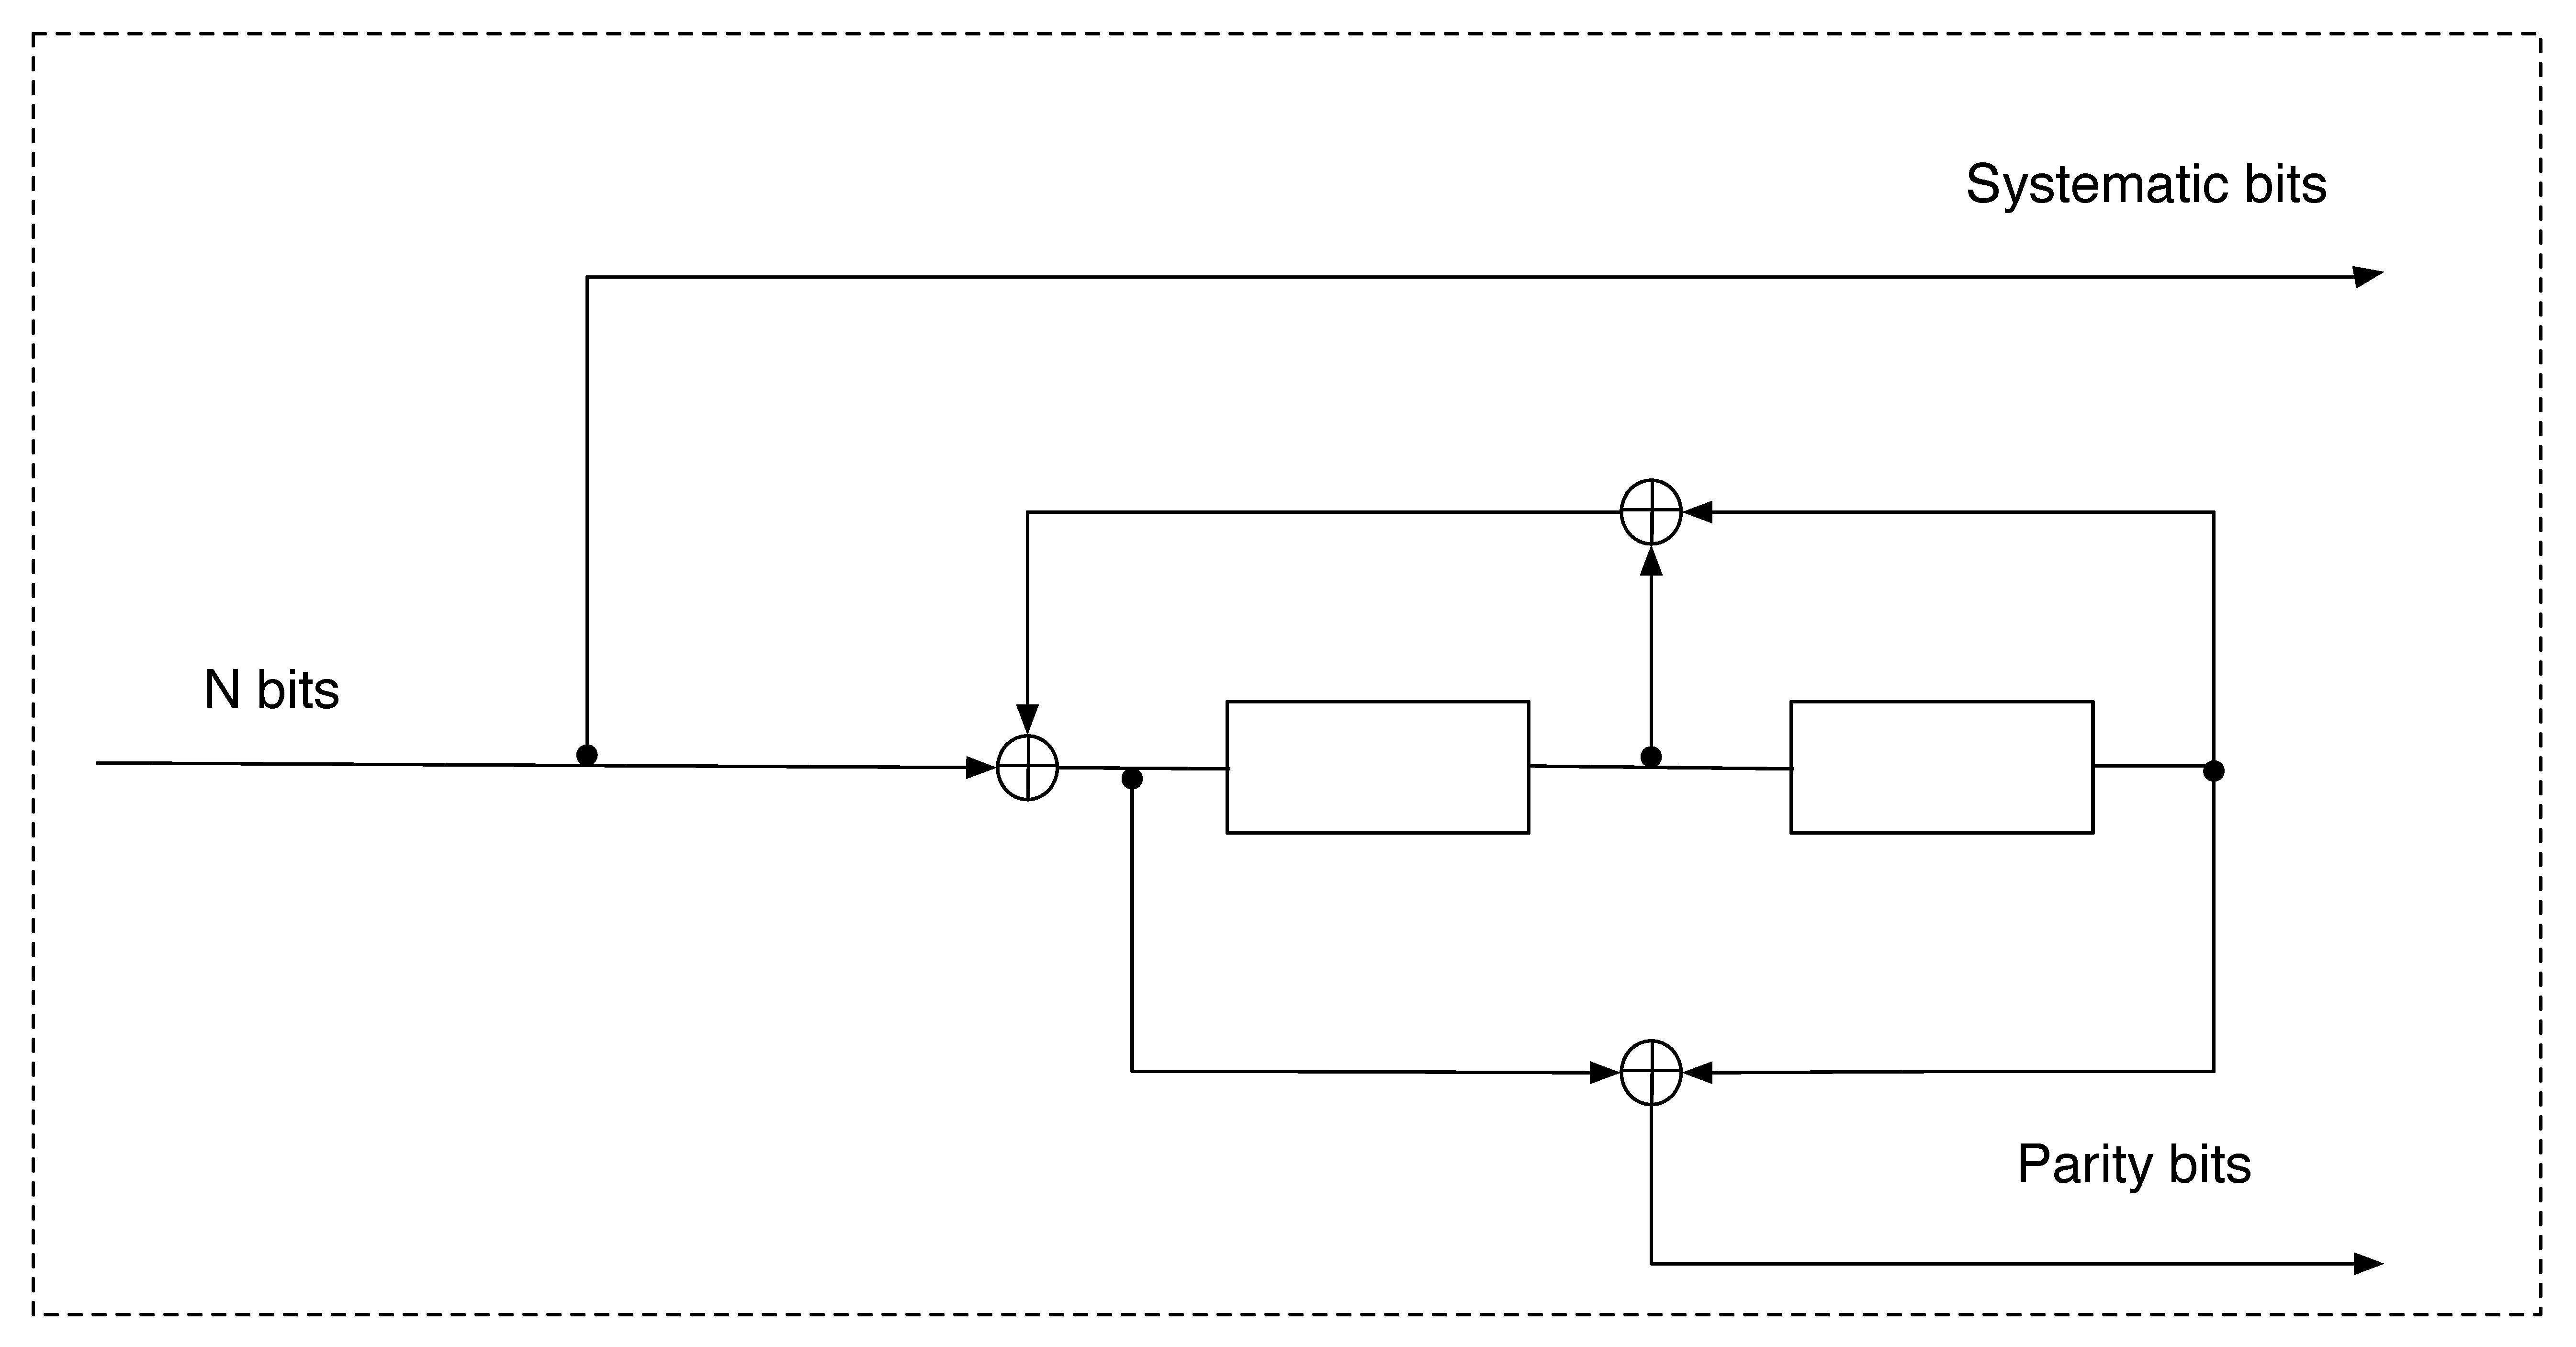
\includegraphics[width=0.45\textwidth]{./PaperSources/RSCExample3.pdf}
		\caption{$[\frac{1+x^2}{1+x+x^2}]$  RSC Encoder}
		\label{fig1}
		\end{figure}
		
A RSC encoder is shown in Figure \ref{fig1} with $k=1$ and $n=2$. Its generator function is given by $[\frac{1+x^2}{1+x+x^2}]$ which may be written as $5/7$ in octal form where $5 ~ \text{and} ~ 7$ correspond to the numerator and denomenator of the generator function respectively. 
 For the $5/7$ RSC code, $\btheta=(1~1~1~ 0~ 1~ 1~ 0~ 1~ 1~ 0~\cdots)$ which may be written in terms of the elements of GF(8) as $\bphi_7~\dot{\bphi_3}$. The corresponding cycle $\bpsi=\bphi_6 $ with a cycle length of $\tau =3$. 
 Moving foward all examples and discussions relating to RSC codes will be done using the $5/7$ RSC code unless otherwise stated.
 %The knowledge of $\textbf{p}$ and $\tau$ will be used in deriving the method for determing which input messages generate low-weight parity bits. 